\documentclass[a4paper,12pt]{article} % тип документа

% Поля страниц
\usepackage[left=2.5cm,right=2.5cm,
    top=2cm,bottom=2cm,bindingoffset=0cm]{geometry}
    
%Пакет дял таблиц   
\usepackage{multirow} 
    
%Отступ после заголовка    
\usepackage{indentfirst}

% Рисунки
\usepackage{floatrow,graphicx,calc}
\usepackage{wrapfig}

%%% Работа с картинками
\usepackage{graphicx}  % Для вставки рисунков
\graphicspath{{images/}}  % папки с картинками
\setlength\fboxsep{3pt} % Отступ рамки \fbox{} от рисунка
\setlength\fboxrule{1pt} % Толщина линий рамки \fbox{}
\usepackage{wrapfig} % Обтекание рисунков и таблиц текстом

% Работа со списками
\renewcommand{\labelitemi}{\textendash}

\usepackage{enumitem}
\setlist[enumerate]{leftmargin=10pt, itemsep=2pt, topsep=2pt}

% Создаём новый разделитель
\DeclareFloatSeparators{mysep}{\hspace{1cm}}

% Ссылки?
\usepackage{hyperref}
\usepackage[rgb]{xcolor}
\hypersetup{				% Гиперссылки
    colorlinks=true,       	% false: ссылки в рамках
	urlcolor=blue          % на URL
}

%  Русский язык
\usepackage[T2A]{fontenc}			% кодировка
\usepackage[utf8]{inputenc}			% кодировка исходного текста
\usepackage[english,russian]{babel}	% локализация и переносы

% Математика
\usepackage{amsmath,amsfonts,amssymb,amsthm,mathtools}

%%% Дополнительная работа с математикой
\usepackage{amsmath,amsfonts,amssymb,amsthm,mathtools} % AMS
\usepackage{icomma} % "Умная" запятая: $0,2$ --- число, $0, 2$ --- перечисление

% Что-то 
\usepackage{wasysym}
\usepackage{verbatim} 


\begin{document}
\begin{center}
	\footnotesize{ФЕДЕРАЛЬНОЕ ГОСУДАРСТВЕННОЕ АВТОНОМНОЕ ОБРАЗОВАТЕЛЬНОЕ 			УЧРЕЖДЕНИЕ ВЫСШЕГО ОБРАЗОВАНИЯ}\\
	\footnotesize{МОСКОВСКИЙ ФИЗИКО-ТЕХНИЧЕСКИЙ ИНСТИТУТ\\(НАЦИОНАЛЬНЫЙ 			ИССЛЕДОВАТЕЛЬСКИЙ УНИВЕРСИТЕТ)}\\
	\footnotesize{ФИЗТЕХ-ШКОЛА ФИЗИКИ И ИССЛЕДОВАНИЙ им. ЛАНДАУ\\}
	\hfill \break
	\hfill \break
	\hfill \break
	\hfill \break
\end{center}

\begin{center}   
    \hfill \break
	\hfill \break
	\hfill \break
	\hfill \break    \hfill \break
	\hfill \break
	\hfill \break
	\hfill \break
    \hfill \break
    \hfill \break
	\hfill \break
	\large{Лабораторная работа № 2.3.1 \\\textbf{Получение и измерение вакуума}}\\
	\begin{flushright}
		Плотникова Анастасия Александровна\\
		Группа Б02-406
	\end{flushright}
	\hfill \break
	\hfill \break
	\hfill \break
\end{center}
\hfill \break
\hfill \break
\hfill \break
\hfill \break
\hfill \break
\hfill \break
\hfill \break
\hfill \break
\hfill \break
\hfill \break
\hfill \break
\hfill \break
\hfill \break
\begin{center}
	Долгопрудный, 2025 г.
\end{center}
\thispagestyle{empty}
\newpage
	\textbf{Цель работы:}\\ 
  1) измерение объёмов форвакуумной и высоковакуумной частей установки; \\
  2) определение скорости откачки системы в стационарном режиме, а также по ухудшению и по улучшению вакуума.
	\hfill \break
	
	\textbf{В работе используются:}\\ 
  вакуумная установка с манометрами: 
  \par масляным,
  \par термопарным ПМТ-2, 2 шт.,
  \par ионизационным ПМИ-2; \\
  вакууметры Мерадат ВИТ16ИТ2, Мерадат ВИТ19ИТ2; \\
  форвакуумный насос; \\
  диффузионный насос; \\
  реостат;
  амперметр;
  соединительные трубки и краны.
	
\section*{Теоретическая справка}

\textbf{Def.} Вакуум — состояние газа, при котором характерная длина свободного пробега сравнима по порядку величины с характерным линейным размером сосуда $d$.

\textbf{Def.} Число Кнудсена — отношение длины свободного пробега $\lambda$ к характерному размеру. Отвечает за критерии применимости законов диффузии, вязкости и теплопроводности.

\begin{equation}
  \text{Kn} = \frac{\lambda}{d}
\end{equation}
$\text{Kn} \ll 1$ — низкий вакуум \\
$\text{Kn} \sim 1$ — средний вакуум \\
$\text{Kn} \gg 1$ — высокий вакуум 

\smallskip

\noindent В обычных лабораторных установках ($d \approx 10$ см): \\
$P > 10^2$ Па (1 торр) — низкий вакуум \\
$10^{-1} < P < 10^2$ Па ($10^{-3}-1$ торр)— средний вакуум \\
$P < 10^{-1}$ Па ($10^{-3}$ торр) — высокий вакуум 

\subsection*{Течение разреженного газа по трубе}

Будет считать газ разреженным настолько, что его молекулы на всех длине трубы $(L, r)$ не сталкиваются между собой и соударяются только со стенкам трубы.

Диаметр трубы $2r$ — среднее расстояние, которое молекула  проходит без соударений. Аналог длины свободного пробега.

Рассмотрим течение разреженного газа через трубу как процесс диффузии с длиной свободного пробега $\lambda = 2r$. 

\begin{equation}
  \label{dN_dt}
  \frac{dN}{dt} = D \frac{dn}{dx} S,
\end{equation}
где $S = \pi r^2$, $D$ — коэффициент диффузии.

\begin{figure}
  \centering
  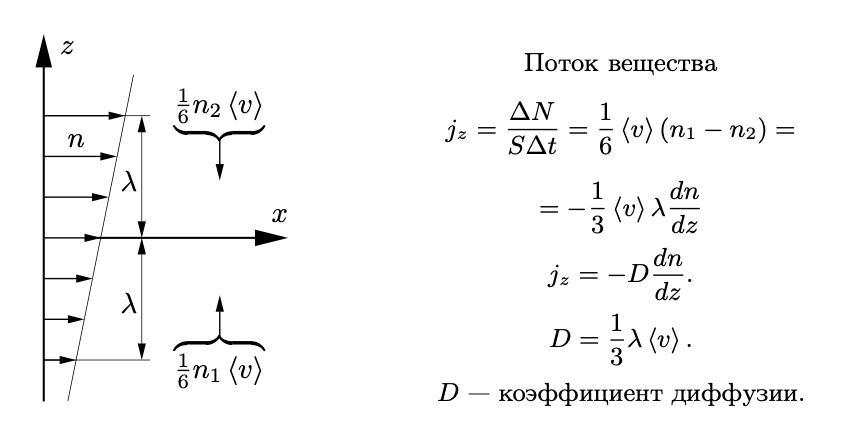
\includegraphics[scale = 0.75]{images/eq.png}
  \caption{Вывод основной формулы явления переноса}
  \label{fig:eq}
\end{figure}

Согласно (\ref{fig:eq}), $D = \lambda \bar{v} / 3$ и $\lambda = 2r$. Получим $D = 2r \bar{v} / 3$. 

Будем использовать среднюю скорость молекул $\bar{v} = \sqrt{\frac{8kT}{\pi m}}$.

При стационарном течении поток постоянен: $dn/dx = \text{const}$. 

Проинтегрируем:

\begin{equation}
  \frac{dn}{dx} = \frac{n_1 - n_2}{L},
\end{equation}
где $n_1$ и $n_2$ — концентрация каза в начале и конце трубы, $L$ — длина трубы.

Подставим в (\ref{dN_dt}). Получим формулу Кнудсена.

\begin{equation}
  \frac{dN}{dt} = \frac{4}{3} r^3 \sqrt{\frac{2 \pi k T}{m}} \frac{n_1 - n_2}{L}
\end{equation}

Используем $dM = mdN$. Масса газа, протекающего в единицу времени через трубу равна:

\begin{equation}
  \frac{dM}{dt} = \frac{4}{3} r^3 \sqrt{2 \pi m k T} \frac{n_1 - n_2}{L}
\end{equation}

Учитывая $P = nkT$:

\begin{equation}
  \frac{dM}{dt} = \frac{4}{3} r^3 \sqrt{\frac{2 \pi m}{k T}}\frac{P_1 - P_2}{L} = \frac{4}{3} r^3 \sqrt{\frac{2 \pi \mu}{R T}}\frac{P_1 - P_2}{L} 
  \label{r3}
\end{equation}
где $P_1$ и $P_2$ — давление газа в начале и конце трубы.

При вакуумных измерениях расход массы иногда вычисляется в единицах $PV$. Связь этой величины с массой следует из формулы Клапейрона:

\begin{equation}
  M = \frac{\mu P V}{R T}
\end{equation}

\begin{equation}
  \frac{d(PV)}{dt} = \frac{4}{3} r^3 \sqrt{\frac{2 \pi R T}{\mu}} \frac{P_1 - P_2}{L}
\end{equation}

Для сравнения с течением вязкого газа при небольших скоростях (по отношению к скорости звука), то есть с течением сплошной среды, используем формулу Пуазейля:

\begin{equation}
  Q = \frac{V}{t} = \int_{0}^{R} v \cdot 2 \pi r dr = \pi \frac{P_1 - P_2}{8 \eta l} R^4
\end{equation}

Коэффициент вязкости $\eta$ в этой формуле выразим через молекулярные параметры газа в соответствии с формулой (\ref{}). В результате формула Пуазейля для сплошной среды будет иметь вид:

\begin{equation}
  \frac{d M}{d t} = \frac{3 \pi}{32} \frac{r^4}{\lambda} \sqrt{\frac{2 \pi m}{k T}} \frac{P_1 - P_2}{L}
  \label{r4}
\end{equation}

Расход сплошной среды пропорционален $r^4$ (\ref{r4}), а разреженной — только $r^3$ (\ref{r3}). 

\subsection*{Адсорбция}

\textbf{Def.} Адсорбцией называется поглощение какого-либо вещества из газообразной среды или раствора поверхностным слоем жидкости или твёрдого тела.

Адсорбция всегда уменьшает коэффициент поверхностного натяжения, то есть свободную поверхностную энергию, иначе адсорбция вообще не происходила бы.

\textbf{Def.} Вещества, способные адсорбироваться на поверхности данной жидкости, называются поверхностно-активными.

\subsection*{Растворы}

\textbf{Def.} Смеси двух или нескольких веществ, в которых эти веще- ства перемешаны молекулярно, называют растворами.

\textbf{Def.} Если одного из веществ в растворе больше, чем других, то его называют растворителем, а остальные — растворенными веществами.

Растворимость одного вещества в другом обычно имеет определённые пределы. 

\textbf{Def.} Раствор, содержащий наибольшее количество вещества, которое можно в нём растворить, называется насыщенным. 

Если к насыщенному раствору добавить ещё некоторое количество вещества, оно уже не будет растворяться. 

\textbf{Def.} Растворимость — концентрация насыщенного раствора. Характеризует способность данного вещества растворяться в данном растворителе. 

\subsection*{Осмотическое давление}

\textbf{Def.} Осмосом называется прохождение растворителя через полупроницаемую перегородку. 

Полупроницаемая перегородка пропускает малые молекулы растворителя, но она непроницаема для более крупных молекул растворенного вещества. 

Осмос всегда идёт от чистого растворителя к раствору и приводит к понижению концентрации. Он продолжается до тех пор, пока вызванное им повышение давления не достигнет определённого предела, которое называется осмотическим давлением.

Осмотическое давление $P_{\text{осм}}$ определяется по формуле, аналогичной формуле для давления идеального газа:
\begin{equation}
  P_{\text{осм}} = nkT,
\end{equation}
где $n$ — число молекул растворенного вещества в единице объёма, \\
$k$ — постоянная Больцмана, \\
$T$ — абсолютная температура.

\subsection*{Вакуумные установки}

По степени разрежения вакуумные установки принято делить на три класса: \\
1) низковакуумные — до $10^{-2}-10^{-3}$ торр; \\ 
2) высоковакуумные — $10^{-4}-10^{-7}$ торр; \\ 
3) установки сверхвысокого вакуума — $10^{-8}-10^{-11}$ торр.

Низкий вакуум переходит в высокий, когда длина свободного пробега молекул газа оказывается сравнима с размерами установки; сверхвысокий вакуум характерен крайней важностью процессов адсорбции и десорбции частиц на поверхности вакуумной камеры.

В данной работе изучаются традиционные методы откачки механическим форвакуумным насосом до давления $10^{-2} $торр и диффузионным масляным насосом до давления $10^{-5}$ торр, а также методы измерения вакуума в этом диапазоне.

\subsection*{Процесс откачки}
\noindent $W = \frac{d V}{d t} \ (\frac{\text{л}}{\text{с}})$ — скорость откачки; \\
$Q_{\text{д}}$ — количество газа, десорбирующегося с поверхности откачиваемого объема в единицу времени; \\
$Q_{\text{и}}$ — количество газа, проникающего в этот объем извне (через щели) в единицу времени; \\
$Q_{\text{и}}$ — поток газа, поступающего из насоса назад в откачиваемую систему. \\

Будем измерять количество газа $Q_{\text{д}}$, $Q_{\text{и}}$ и $Q_{\text{н}}$ в единицах $PV$.

\begin{equation}
  - d(PV) = -PdV - V dP = -VdP = (P W - Q_{\text{д}} - Q_{\text{и}} - Q_{\text{н}})dt
  \label{eq1}
\end{equation}


Левая часть этого уравнения равна убыли газа в откачиваемом объёме $V$ , а правая определяет количество газа, уносимого насосом, и количество прибывающего вследствие перечисленных выше причин за время $dt$. При достижении предельного вакуума (давления $P_{\text{пр}}$): \( dP/dt = 0 \).

\begin{equation}
  P_{\text{пр}} W = Q_{\text{д}} + Q_{\text{и}} + Q_{\text{н}}
  \label{eq2}
\end{equation}

Обычно $Q_{\text{и}}$ постоянно, a $Q_{\text{н}}$ и $Q_{\text{д}}$ слабо зависят от времени, поэтому в наших условиях все эти члены можно считать постоянными. Считая также постоянной скорость откачки $W$, уравнение (\ref{eq1}) можно проинтегрировать. Используем (\ref{eq2}):

\begin{equation}
  -VdP = (P W - P_{\text{пр}} W)dt  = (P - P_{\text{пр}}) Wdt 
\end{equation}
\begin{equation}
  \int^{P}_{P_0}\frac{dP}{P - P_{\text{пр}}} = - \int^{t}_{0} \frac{W}{V} dt
\end{equation}
\begin{equation}
  \ln\frac{P - P_{\text{пр}}}{P_0 - P_{\text{пр}}} = - \frac{W}{V} t
\end{equation}
\begin{equation}
  P - P_{\text{пр}} = (P_0 - P_{\text{пр}}) e^{\frac{W}{V}}
\end{equation}
$P_0$ обычно велико по сравнению с $P_{\text{пр}}$:
\begin{equation}
  P = P_0 e^{- \frac{W}{V}}
\end{equation}

\subsection*{Течение газа через трубу}

Характер течения газа существенно зависит от соотношения между размерами системы и длиной свободного пробега молекул.

Для количества газа, протекающего через трубу в условиях высокого вакуума, или, как говорят, в кнудсеновском режиме, справедлива формула:
\begin{equation}
  \frac{d(PV)}{dt} = \frac{4}{3} r^3 \sqrt{\frac{2 \pi R T}{\mu}} \frac{P_1 - P_2}{L}
\end{equation}

В случае, когда труба соединяет установку с насосом, $P_1 \ll P_2 = P$.
\begin{equation}
  C_{\text{тр}} = \left( \frac{dV}{dt} \right)_{\text{тр}} = \frac{4}{3} \frac{r^3}{L} \sqrt{\frac{2 \pi R T}{\mu}} 
\end{equation}
Поэтому в вакуумных установках следует применять широкие и короткие трубы.

Пропускная способность отверстий:
\begin{equation}
  \nu = \frac{1}{4} Sn \langle v \rangle,
\end{equation}
где $\nu = dN/dt$ в вакуум, \\
$n$ — концентрация молекул перед отвертстием.\\
\begin{equation}
  \nu = dN/dt, \quad N = PV/kT, \quad n = P/kT
\end{equation}
\begin{equation}
  C_{\text{отв}} = S \frac{\langle v \rangle}{4}
\end{equation}

\section*{Экспериментальная установка}

Схема установки изображена на рисунке (\ref{fig:setup}). 

\medskip

\begin{figure}[h]
  \centering
  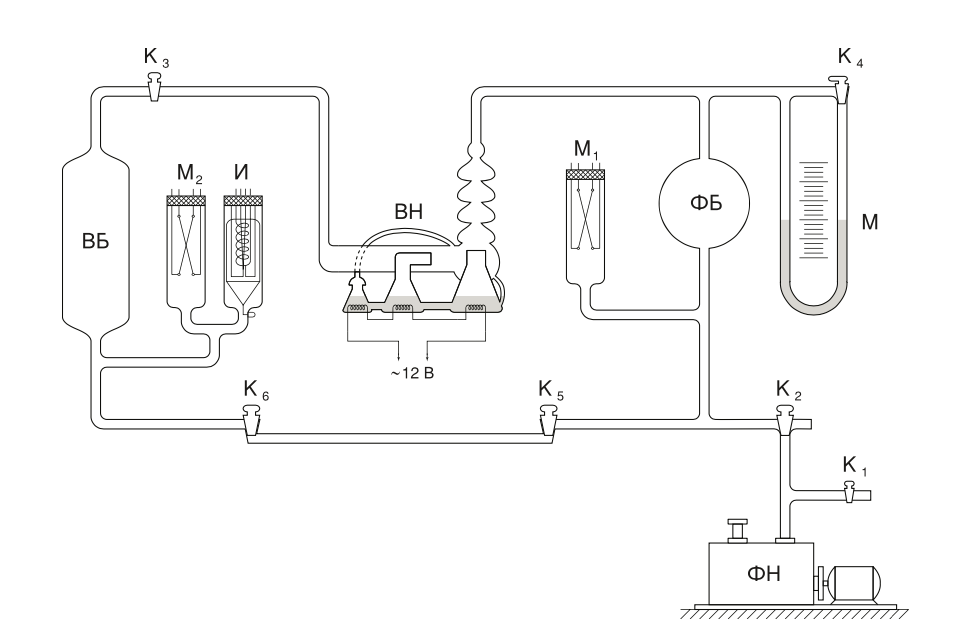
\includegraphics[scale = 1]{images/setup.png}
  \caption{Схема экспериментальной установки}
  \label{fig:setup}
\end{figure}

Установка изготовлена из стекла и состоит из: \\ 
— форвакуумного баллона (ФБ), \\ 
— высоковакуумного диффузионного насоса (ВН), \\ 
— высоковакуумного баллона (ВБ), \\ 
— масляного (М) и ионизационного (И) манометров, \\ 
— термопарных манометров (М1 и M2), \\ 
— форвакуумного насоса (ФН), \\ 
— соединительных кранов К1, К2, ..., К6. 

Кроме того, в состав установки входят: \\ 
— вариатор (автотрансформатор с регулируемым выходным напряжением) или реостат, \\ 
— амперметр для регулирования тока нагревателя диффузионного насоса.

\subsection*{Краны}

Все краны вакуумной установки — стеклянные.

Для герметизации используется вакуумная смазка. 

Если на поверхности шлифа видны круговые полосы, то кран либо плохо притёрт, либо неправильно смазан и может пропускать воздух. 

Краны работают лишь в том случае, если давление внутри крана меньше атмосферного. При этом пробка вдавливается внутрь крана.

\subsection*{Форвакуумный насос} 

Устройство и принцип действия ротационного пластинчатого форвакуумного насоса схематически показаны на рис. (\ref{fig:pre-vacuum_pump}).

\begin{figure}[h]
  \centering
  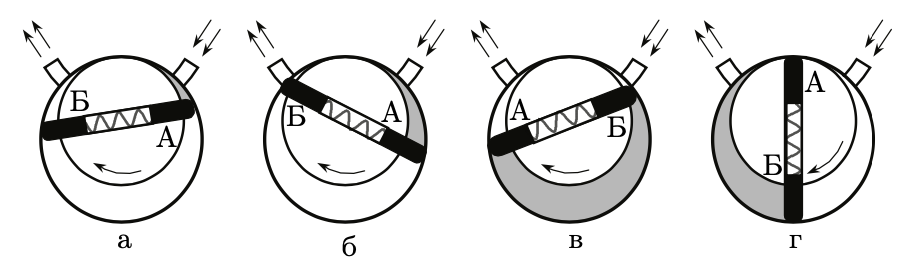
\includegraphics[scale = 0.75]{pre-vacuum_pump.png}
  \caption{\centering Схема действия ротационного двухпластинчатого форвакуумного насоса. В положениях «а» и «б» пластина «А» засасывает разреженный воздух из откачиваемого объёма, а пластина «Б» вытесняет ранее захваченный воздух в атмосферу. В положениях «в» и «г» пластины поменялись ролями}
  \label{fig:pre-vacuum_pump}
\end{figure}

В цилиндрической полости массивного корпуса размещен эксцентрично ротор так, что он постоянно соприкасается своей верхней частью с корпусом. В диаметральный разрез ротора вставлены две пластины, раздвигаемые пружиной и плотно прижимаемые к поверхности полости.

Они разделяют объём между ротором и корпусом на две части. Действие насоса ясно из изображённых на рис. (\ref{fig:pre-vacuum_pump}) последовательных положений пластин при вращении ротора по часовой стрелке. 

При работе с насосом следует помнить, что после остановки насоса в него обязательно нужно впускать воздух. Если этого не делать, то атмосферное давление может выдавить масло из насоса в патрубки и в вакуумную систему. Соединять насос с атмосферой следует при помощи кранов $K1$ или $K2$.

После включения насоса его присоединяют к установке не сразу, а через некоторое время, когда насос откачает собственный объём и пространство, расположенное до крана К2. Об этом можно судить по звуку насоса. Вначале насос сильно шумит, затем его звук делается мягким, и, наконец, в насосе возникает сухой стук, — это происходит, когда достигается хорошее разрежение.

\subsection*{Диффузионный насос}

Откачивающее действие диффузионного насоса основано на диффузии (внедрении) молекул разреженного воздуха в струю паров масла. 

Попавшие в струю молекулы газа увлекаются ею и уже не возвращаются назад. На прежнем их месте образуется пустота, которая немедленно заполняется следующими порциями газа, увеличивая степень разрежения газа в окрестности струи и оказывая таким образом сильное откачивающее воздействие на весь газ в откачиваемом объёме. 

Скорость откачки диффузионных насосов в сотни и тысячи раз превосходит скорость откачки форвакуумного насоса.

Устройство одной ступени масляного диффузионного насоса схематически показано на рис. (\ref{fig:diffusion_pump}).

\begin{figure}[h]
  \centering
  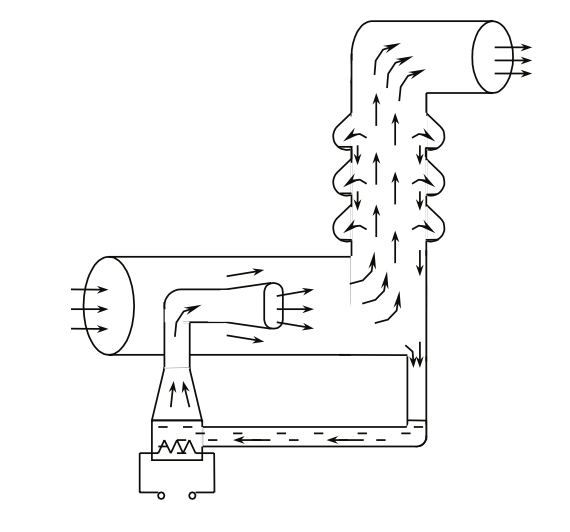
\includegraphics[scale = 0.75]{diffusion_pump.png}
  \caption{Схема работы диффузионного насоса}
  \label{fig:diffusion_pump}
\end{figure}

Масло, налитое в сосуд А, подогревается электрической печкой. Пары масла поднимаются по трубе Б и вырываются из сопла В. Струя паров увлекает молекулы газа, которые поступают из откачиваемого сосуда через трубку ВВ. Дальше смесь попадает в вертикальную трубу Г. Здесь масло осаждается на стенках трубы и маслосборников и стекает вниз, а оставшийся газ через трубу ФВ откачивается форвакуумным насосом. 

Диффузионный насос работает наиболее эффективно при давлении, когда длина свободного прбега молекул воздуха примерно равна ширине кольцевого зазора между соплом В и стенками трубы ВВ. 

Если диффузионный насос включить при давлении, сравнимом с давлением насыщенного пара масла, то последнее никакой струи не создаст и масло будет просто окисляться и угорать.

Граничное давление, выше которого диффузионный насос включать нельзя, на вакуумметрах термопарных ламп отмечено красной линией ($\sim 1,2$ мВ).

\medskip 

Диффузионный насос, используемый в нашей установке (рис. 1), имеет две ступени и соответственно два сопла. Одно сопло вертикальное (первая ступень), второе сопло горизонтальное (вторая ступень). 

За второй ступенью имеется ещё одна печь, она осуществляет фракционирование масла. Легколетучие фракции масла, испаряясь, поступают в первую ступень. По этой причине плотность струи первой ступени выше, и эта ступень начинает откачивать газ при более высоком давлении в форвакуумной части установки. Вторая ступень обогащается малолетучими фракциями. Плотность струи второй ступени меньше, но меньше и давление насыщенных паров масла в этой ступени. 

Соответственно в откачиваемый объём поступает меньше паров масла, и его удаётся откачать до более высокого вакуума.

\medskip

При работе с диффузионным насосом необходимо придерживаться следующих правил:
\begin{itemize}
  \item Включать подогрев диффузионного насоса можно лишь после того, как вакуум в системе доведен до $5 \cdot 10^{-2}$ торр при помощи форвакуумного насоса. При недостаточном предварительном разрежении масло в диффузионном насосе портится.
  \item Не следует допускать слишком интенсивного кипения масла.
\end{itemize}

\subsection*{Масляный манометр}

Заполнен вязкой жидкостью с очень низким давлением насыщенных паров. Из-за большой вязкости масла уровни в манометре устанавливаются не сразу.

Во время откачки и заполнения установки атмосферным воздухом кран $K_4$ должен быть открыт во избежание выброса масла. 

\subsection*{Термопарный манометр}

Чувствительный элемент – термопара, спаянная с никелевой нитью накала и заключённая в стеклянный баллон (лампа ЛТ-2 или ПМТ-2).

\begin{figure}[h] % Размещение справа, ширина области 45% от текста
  \centering
  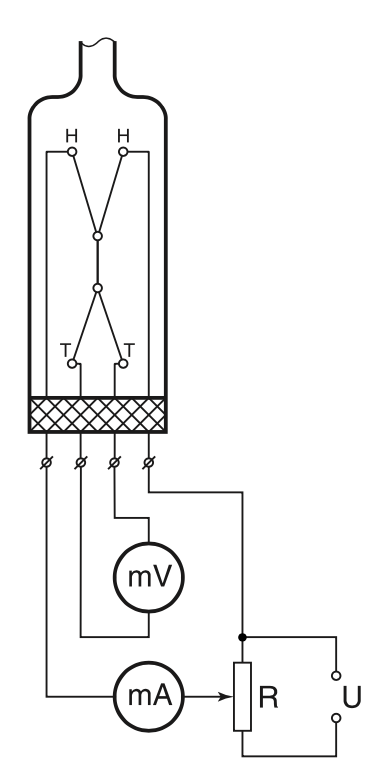
\includegraphics[scale = 0.5]{thermo_scheme.png}
  \caption{Схема термопарного манометра}
  \label{fig:thermo_scheme}
\end{figure}

Использует зависимость теплопроводности газов от давления в определенном диапазоне, которая представлена на рисунке (\ref{fig:thermo}).

\begin{figure}[h!]
  \centering
  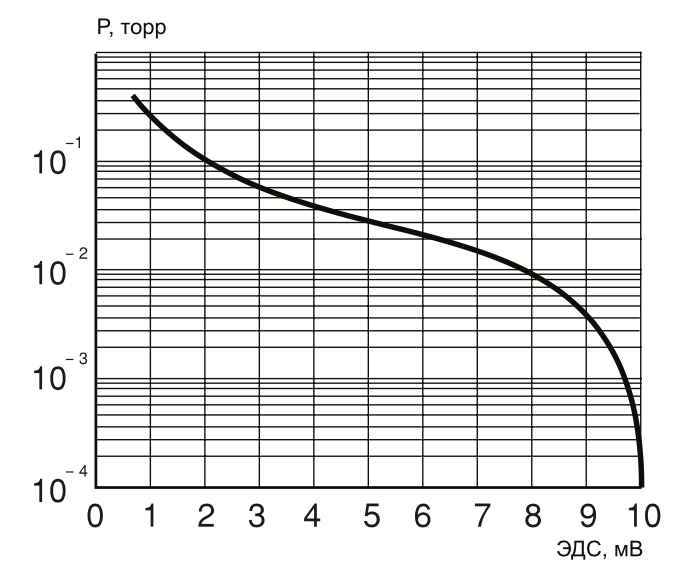
\includegraphics[scale = 0.5]{thermo.png}
  \caption{Градуировочная кривая термопары ЛТ-2}
  \label{fig:thermo}
\end{figure}

\subsection*{Ионизационный манометр}

Представляет собой трёхэлектродную лампу.

Ионный ток в цепи коллектора пропорционален плотности газа и поэтому может служить мерой давления.

\begin{figure}[h!]
  \centering
  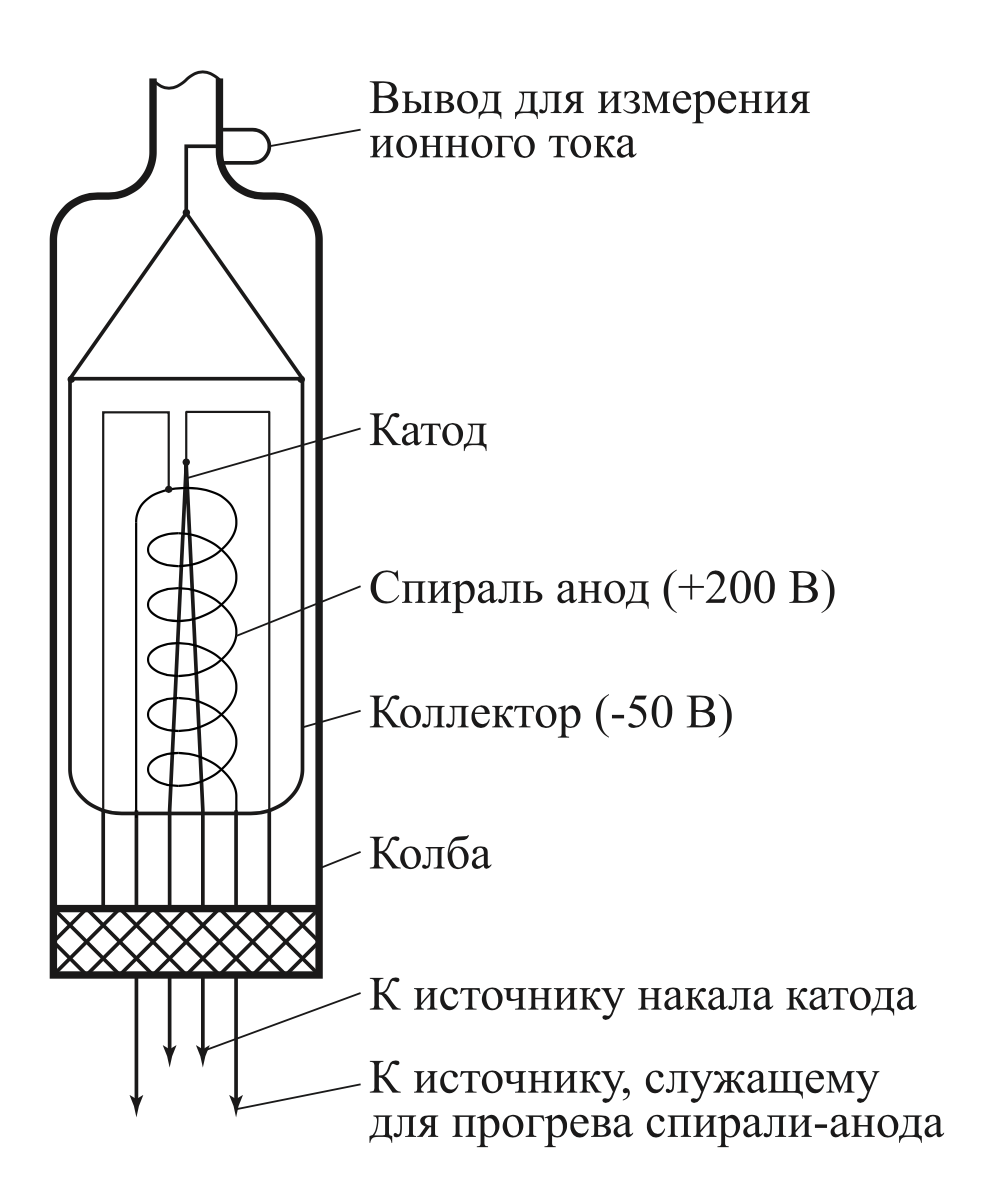
\includegraphics[scale = 0.3]{ion.png}
  \caption{Схема ионизационного манометра}
  \label{fig:ion}
\end{figure}

\section*{Ход работы}

\begin{center}
  \textsf{I. Определение объёма форвакуумной и высоковакуумной частей установки}
\end{center}

\begin{enumerate}

  \item Проверим, что кран $K_4$ открыт. Откройте все краны, кроме $K_1$ и $K_2$. 
  \item Впустим в установку атмосферный воздух через краны $K_1$ и $K_2$.
  \item Запрем воздух в капилляре, закрыв краны $K_5$ и $K_6$. Объем запертого воздуха при атмосферном давлении равен $V = (50 \pm 1) \, \text{см}^3$.
  \item Закроем краны $K_1$ и $K_2$, включим форвакуумный насос и дадим ему откачать себя. Затем, открыв $K_2$, откачаем установку до давления $10^{-2}$ торр. Давление будем измерять вакуумметром ВТ-2, соединённым с лампой $M_1$. 
  \item Повернув рукоятку крана $K_2$, отсоединиv установку от форвакуумного насоса. Выключив насос, откроем $K_1$ на атмосферу.
  \item Перекрыв кран $K_3$, отделим высоковакуумную часть установки от форвакуумной.
  \item Закроем $K_4$, кран масляного манометра.
  \item Откроем капилляр в форвакуумную часть ($K_5$). Запертый воздух распространится по всему объёму форвакуумной части установки и повысит в ней давление.
  
  Дождемся установления показаний манометра, измерим уровни масла $h_1^{\text{фв}}$ и $h_2^{\text{фв}}$.
  
  \item Зная объём запертого воздуха (см. п. 3), найдем объём $V_{\text{фв}}$ форвакуумной части по закону Бойля–Мариотта, полагая значение давления при вакууме много меньше атмосферного.
  
  \begin{equation}
    p_{\text{полн}} = \rho g |h_{1} - h_{2}| = \rho g \Delta h, \qquad \rho = (0.885 \pm 0.001) \, \frac{\text{г}}{\text{см}^3}
  \end{equation}
  \begin{equation}
    p_{\text{фв}} V_{\text{фв}} = p_{\text{вв}} (V_{\text{фв}} + V_{\text{вв}}) = p_0 V_0
  \end{equation}
  \begin{equation}
    V_{\text{фв}} = \frac{p_0 V_0}{\rho g \Delta h^{\text{фв}}}
  \end{equation}
  
  \begin{table}[h]
    \caption{}
    \begin{tabular}{|c|c|c|c|}
        \hline $h_1^{\text{фв}}$, мм  &  $h_2^{\text{фв}}$, мм & $\Delta h^{\text{фв}}$, мм  &  $V_{\text{фв}}$, см$^3$ \\
        \hline
        347 & 93  & 254 & 2215 \\
        350 & 96  & 254 & 2215 \\
        \hline 
    \end{tabular}
    \label{tab:pv_data}
  \end{table}
  
  \item Соединим форвакуумную и высоковакуумную части, открыв $K_3$. Вновь дождемся установления показаний манометра и измерим уровни масла $h_1^{\text{вв}}$ и $h_2^{\text{вв}}$.
  
  Рассчитаем полный объём установки и объём высоковакуумной её части $V_{\text{вв}}$.
  
  \begin{equation}
    V_{\text{вв}} = \frac{p_0 V_0}{\rho g \Delta h^{\text{вв}}} - V_{\text{фв}}
  \end{equation}
  
  \begin{table}[h]
    \caption{}
    \begin{tabular}{|c|c|c|c|}
        \hline $h_1^{\text{вв}}$, мм  &  $h_2^{\text{вв}}$, мм & $\Delta h^{\text{вв}}$, мм  &  $V_{\text{вв}}$, см$^3$ \\
        \hline
        305 & 142 & 163 & 1265 \\
        305 & 143 & 162 & 1286  \\
        \hline 
    \end{tabular}
    \label{tab:hv_data}
  \end{table}

  Получается:
  \begin{equation}
    V_{\text{фв}} = (2215 \pm 12) \, \text{см}^3, \quad V_{\text{вв}} = (1280 \pm 40) \, \text{см}^3
  \end{equation}

  При всех расчетах погрешностей считаем $\sigma_h = 1$ мм.

  \item Откроем $K_4$.
  \item Измерения по пп. 1–10 повторим ещё раз.

\begin{center}
  \textsf{II. Получение высокого вакуума и измерение скорости откачки}
\end{center}

    \item Откачаем установку форвакуумным насосом. Убедимся в том, что краны в установке повёрнуты так, что в ней не осталось запертых объёмов.
    \item Включим термопарный манометр в высоковакуумной части установки и не будем выключать его до конца работы. Наблюдаем показания на соответсвующем вакууметре.
    \item После того как давление упадёт ниже $10^{-2}$ торр, перекроем капилляр $K_6$. Плавно увеличим ток до предельно допустимого на нагрев масла в диффузионном насосе (чтобы не пенилось в процессе), затем начнем высоковакуумную откачку.
    \item Когда значение давления достигнет $2 \cdot 10^{-5}$ торр, включим ионизационный манометр. Проведем дегазацию. 
    \item Запишем предельное значение давления: $P = 8.1 \cdot 10^{-5}$ торр.
    \item Найдём скорость откачки по улучшению вакуума во время откачки. Для этого:
    \begin{enumerate}
        \item отключим откачку высоковакуумного баллона краном $K_3$ и подождём, пока вакуум ухудшится до \( 6 \cdot 10^{-5} \) торр;
        \item откроем кран $K_3$ и отметим изменение показаний ионизационного манометра во времени;
        \item изобразим полученные результаты на графиках $P(t)$ для ухудшения вакуума (см. рис. (\ref{fig:worse})) и \( \ln \frac{P - P_p}{P_0 - P_p} (t) \) для улучшения (см. рис. (\ref{fig:better})). 
        
        Графике ухудшения вакуума с большой точностью апроксимируется прямой. Коэффициент наклона будет равен потоку десорбции и течей $k^w = Q_\text{д}/V_\text{вв}$.

        \begin{figure}[h!]
          \centering
          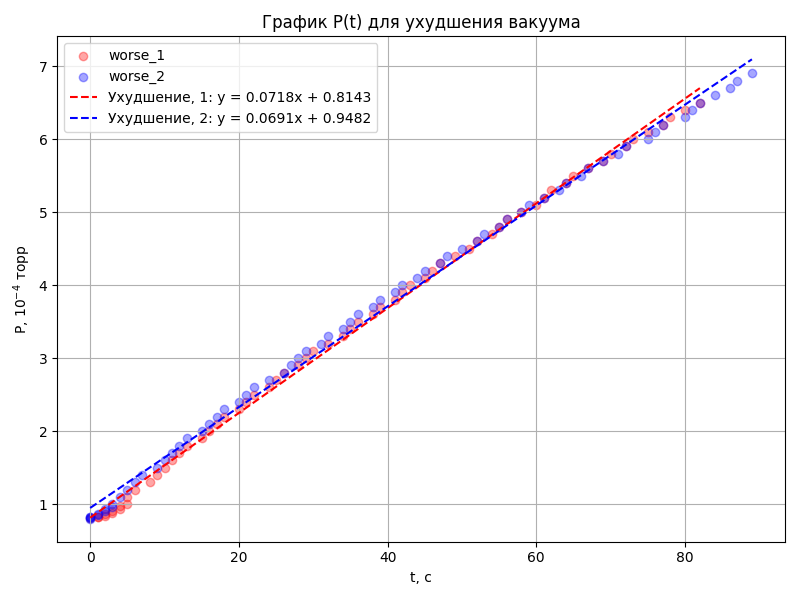
\includegraphics[scale = 0.75]{graph_worse.png}
          \caption{График $P(t)$ ухудшения вакууума}
          \label{fig:worse}
        \end{figure}
        
        Воспользуемся методом наименьших квадратов и получим угловые коэффициенты для обоих наборов данных.

        Учтём погрешности прямых измерений ($dk^w_{{\text{изм}}} = 0.7 \cdot 10^{-6} \, \frac{\text{торр}}{\text{с}}$) и погрешности МНК ($dk^w_{1_{\text{МНК}}} = 0.04 \cdot 10^{-6} \, \frac{\text{торр}}{\text{с}}$ и $dk^w_{2_{\text{МНК}}} = 0.05 \cdot 10^{-6} \, \frac{\text{торр}}{\text{с}}$). 
        
        Получим:
        \begin{equation}
          k^w_1 = (7.2 \pm 0.7) \cdot 10^{-6} \, \text{торр}/\text{с},
        \end{equation}
        \begin{equation}
          k^w_2 = (7.0 \pm 0.7) \cdot 10^{-6} \, \text{торр}/\text{с},
        \end{equation}
        \begin{equation}
          k^w = (7.1 \pm 0.8) \cdot 10^{-6} \, \text{торр}/\text{с}.
        \end{equation}
        
        Рассчитаем $Q_\text{д}$.
        \begin{equation}
          Q_\text{д} = k^w V_\text{вв} = (7.1 \pm 0.8) \cdot 10^{-6} \, \frac{\text{торр}}{\text{с}} \ \cdot (1.28 \cdot 0.04) \, \text{л} = (9.0 \pm 1.2) \, \frac{\text{торр·л}}{\text{с}}
        \end{equation}
        
        График улучшения вакуума апроксимируется прямой заметно хуже. Вероятно, это связано с тем, что мы пользуемся не истинным предельным давлением, а достижимым в эксперименте. При построении прямой не будем учитывать последние три точки из каждого набора данных, так как они заметно выбиваются из общей картины. 
        
        Из теоретической справки известно, что угловой коэффициент будет равен $k^b = -W/V$.
        \begin{equation}
          \ln\frac{P - P_{\text{пр}}}{P_0 - P_{\text{пр}}} = - \frac{W}{V} t
        \end{equation}

        \begin{figure}[h!]
          \centering
          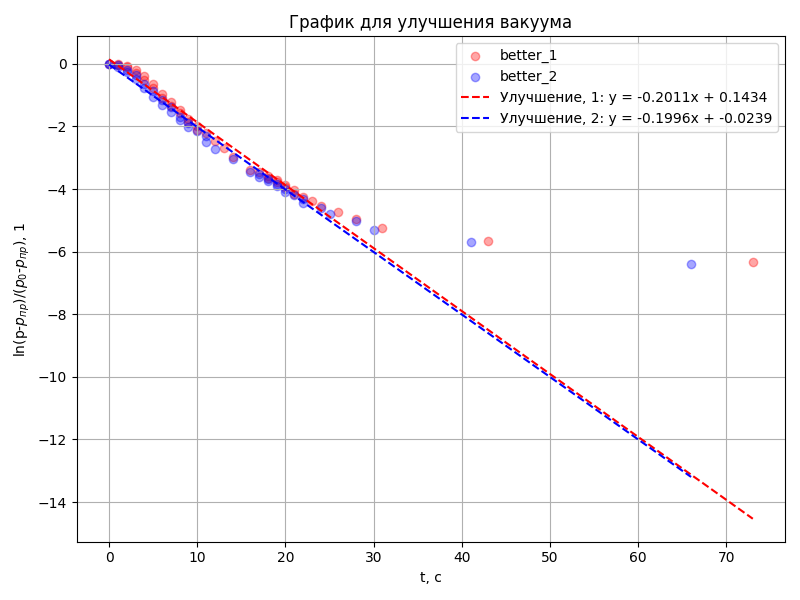
\includegraphics[scale = 0.75]{graph_better.png}
          \caption{График улучшения вакууума}
          \label{fig:better}
        \end{figure}

        Воспользуемся методом наименьших квадратов и получим угловые коэффициенты для обоих наборов данных.

        Учтём погрешности МНК ($dk^w_{1_{\text{МНК}}} = 0.03 \cdot 10^{-1} \, 1/\text{с}$ и $dk^w_{2_{\text{МНК}}} = 0.02 \cdot 10^{-1} \, 1/\text{с}$). 
        \begin{equation}
          k^b_1 = -(2.01 \pm 0.03) \cdot 10^{-1} \, 1/\text{с},
        \end{equation}
        \begin{equation}
          k^b_2 = -(2.00 \pm 0.03) \cdot 10^{-1} \, 1/\text{с},
        \end{equation}

        Учтём погрешность измерений. Погрешность давления зависит от значения и диапазона и равна единице последнего разряда прибора, т.е 0.1 или 0.01 торр.
        \begin{equation}
          \varepsilon(ln(\dots)) = \left\langle \frac{\sqrt{\frac{\Delta P^2 + \Delta P_p^2}{(P - P_p)^2} + \frac{\Delta P_0^2 + \Delta P_p^2}{(P_0 - P_p)^2}}}{\ln \frac{P - P_p}{P_0 - P_p}} \right\rangle = 0.12
        \end{equation}
        
        Получим:
        \begin{equation}
          k^b = -(2.0 \pm 0.4) \cdot 10^{-1} \, 1/\text{с}.
        \end{equation}

        \item рассчитаем \( W \) системы.
        
        \begin{equation}
          W = -k^b \cdot V_{\text{вв}} = 0.26 \text{л}/\text{с}
        \end{equation}
        \begin{equation}
          \varepsilon_W = \sqrt{\varepsilon_{k^b}^2 + \varepsilon_{V_{\text{вв}}}^2} = 0.16
        \end{equation}
        
        \begin{equation}
          W = (0.26 \pm 0.04) \, \text{л/с} = (2.6 \pm 0.4) \cdot 10^{-1} \, \text{л/с} 
        \end{equation}
    \end{enumerate}
    
    \item Оценим величину потока \( Q_{\text{н}} \). Для этого:
    \begin{enumerate}
        \item Перекроем $K_3$, прекратив откачку высоковакуумной части системы. При помощи ионизационного вакуумметра и секундомера будем следить за тем, как ухудшается вакуум. Опыт прекратим, когда давление в системе станет близким к предельному. В этот момент откроем $K_3$, чтобы не пережечь ионизационный манометр;
        \item Используя значение \( W \), найденное в п. 18, и учтя, что уравнение (1) для этого случая принимает вид \(V_{\text{вв}} dP = (Q_{\text{д}} + Q_{\text{и}}) dt,\) оценим \( Q_{\text{н}} \).
        \begin{equation}
          Q_{\text{н}} = (1.1 \pm 0.4) \cdot 10^{-5} \, \text{торр·л}/\text{с}
        \end{equation}

    \end{enumerate}

    \item Проведем повторные измерения по пунктам 18 и 19. Их результаты приведены (на графиках, так как точек много) и проанализированы выше.

    \begin{comment}
      Производительность насоса по различию \( P_{\text{уст}} \) и \( P_{\text{пр}} \). Для этого найдем количество газа, протекающего через капилляр, по формуле (6). Запишем формулу (2) для случаев, когда капилляр перекрыт и когда он открыт:
      \[
      P_{\text{пр}} W = Q_1, \quad P_{\text{уст}} W = Q_1 + \frac{d(PV)_{\text{капилл}}}{dt}
      \]
      В этих формулах символом \( Q_1 \) обозначена сумма всех натеканий, кроме натекания через искусственную течь. Исключим из этих формул натекание \( Q_1 \) и найдем скорость откачки системы (в том сечении, где присоединен манометр).
      Сравним получившееся значение \( W \) с полученным в п. 18. Прокомментируем причины возможного их несовпадения.
    \end{comment}

    \item Выключим установку. Для этого:
    \begin{enumerate}
        \item Выключим накал ионизационного манометра и дадим его лампе остыть примерно 1–2 мин;
        \item Выключим подогрев диффузионного насоса, подождем, пока масло в диффузионном насосе остынет ($\sim$10 минут);
        \item Краном К2 отсоединим установку от форвакуумного насоса, не сообщая её с атмосферой;
        \item Удостоверимся, что показания термопарных манометров М1 и М2 совпадают. Если они различаются, то отрегулируем манометр М1 по показаниям термовакуумметра М2, уже откалиброванного при высоком вакууме;
        \item Выключим форвакуумный насос и, когда он остановится, соединим его с атмосферой краном К1, не напуская атмосферу в установку;
        \item Выключим вакуумметры тумблерами «Сеть».
    \end{enumerate}
\end{enumerate}

\section*{Вывод}

Все цели работы достигнуты.

\begin{enumerate}
  \item Объёмы форвакуумной и высоковакуумной частей установки измерены с помощью закона Бойля–Мариотта.
  \begin{equation}
    V_{\text{фв}} = (2215 \pm 12) \, \text{см}^3, \quad V_{\text{вв}} = (1280 \pm 40) \, \text{см}^3
  \end{equation}
  \item Скорость откачки системы в стационарном режиме, а также по ухудшению вакуума (при перекрытом насосе и наличии течей) и по улучшению вакуума (в процессе откачки), измерена. Результаты представлены в II части работы.
  
	\hfill \break
\end{enumerate}


\end{document}

